\section{Side-by-side}
\label{sec:sbs}

As a viewer's reference note, the theoretical values are presented on the left and the simulation values on the right.
%Esquerda sao sempre valores teoricos, direita valores do Ngpsic

\begin{table}[h]
\begin{center}
  \begin{tabular}{|c|c|}
    \hline    
    {\bf Name} & {\bf Value [Hz]} \\ \hline
    $Z_{I1}$ & 640.4922\\ \hline
$Z_{O1}$ & 477.0475\\ \hline
$AV_{1}$ & 110.6998\\ \hline
$Z_{I2}$ & 15013.86\\ \hline
$Z_{O2}$ & 0.9327305\\ \hline
$AV_{2}$ & 0.9856738\\ \hline

    \hline
  \end{tabular}
  \begin{tabular}{|c||c|}
    \hline    
    {\bf Name} & {\bf Value [Hz]} \\ \hline
    uco & 3.106930e+06\\ \hline
lco & 7.923603e+00\\ \hline
bandwith & 3.106922e+06\\ \hline

    \hline
  \end{tabular}
  \caption{Comparison 1}
  \label{tab:comparison 1}
\end{center}
\end{table}
\FloatBarrier

\begin{table}[h]
\begin{center}
  \begin{tabular}{|c|c|}
    \hline    
    {\bf Name} & {\bf Value [dB]} \\ \hline
    $Z_{I}$ & 640.4922\\ \hline
$Z_{O}$ & 2.9364\\ \hline
$AV$ & 107.21838\\ \hline

    \hline
  \end{tabular}
  \begin{tabular}{|c||c|}
    \hline    
    {\bf Name} & {\bf Value [dB]} \\ \hline
    z_in1 & 5.638527e+02,-8.44302e+01\\ \hline
gain & -7.85216e+01,-1.54185e+00\\ \hline
lco & 8.880418e+03\\ \hline
uco & 1.603742e+06\\ \hline
bandwith & 1.594862e+06\\ \hline
cost & 1.013002e+05\\ \hline
merit & -1.39209e-01,-2.73352e-03\\ \hline

    \hline
  \end{tabular}
  \caption{Comparison 2}
  \label{tab:comparison 2}
\end{center}
\end{table}
\FloatBarrier

\begin{figure}[h] \centering
\includegraphics[scale=0.35]{teo_gain.eps}
\includegraphics[scale=0.27]{vo1f.pdf}
\caption{Output voltage gain in order to frequency}
\label{fig:comparison 3}
\end{figure}
\FloatBarrier

\begin{figure}[h] \centering
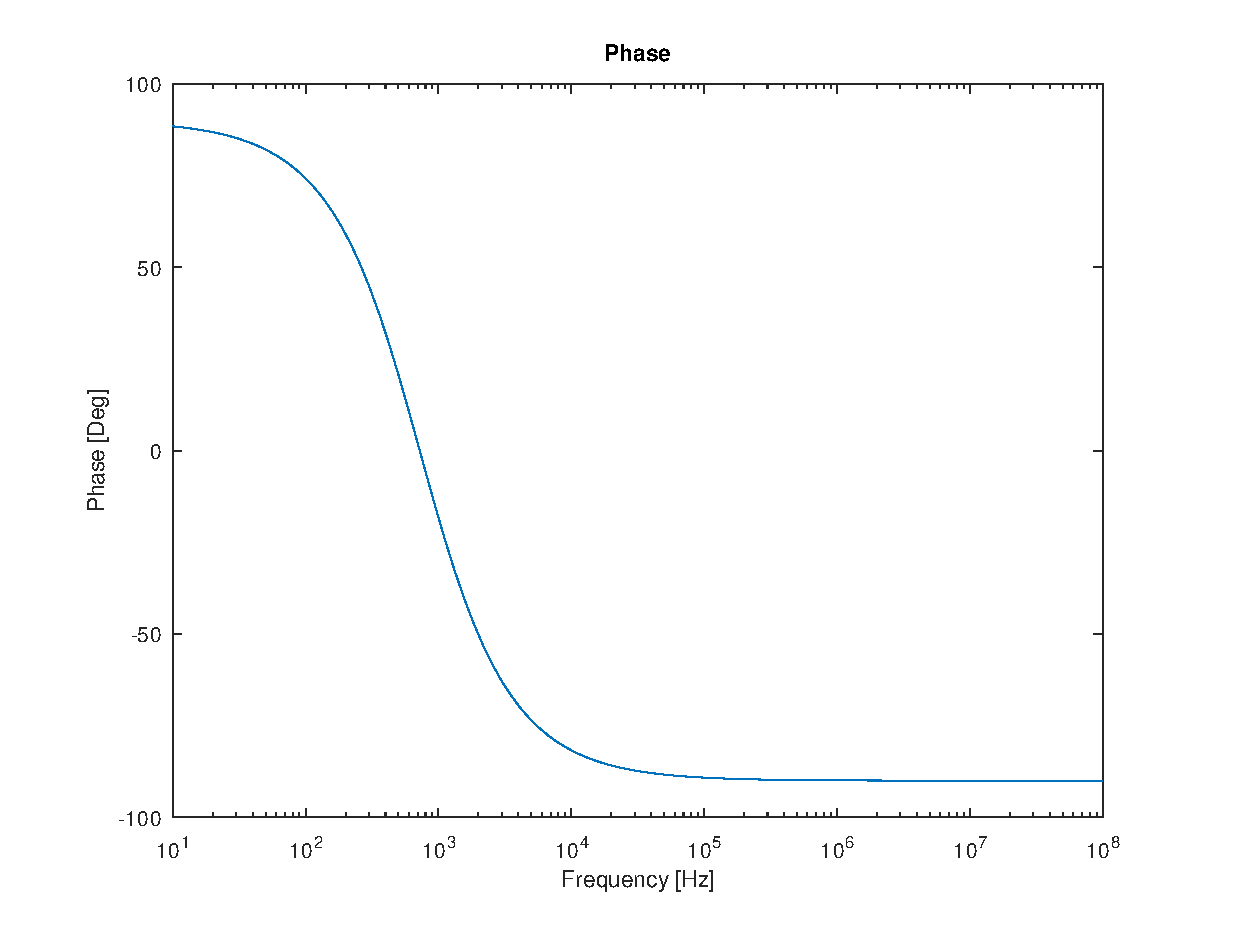
\includegraphics[scale=0.35]{teo_phase.eps}
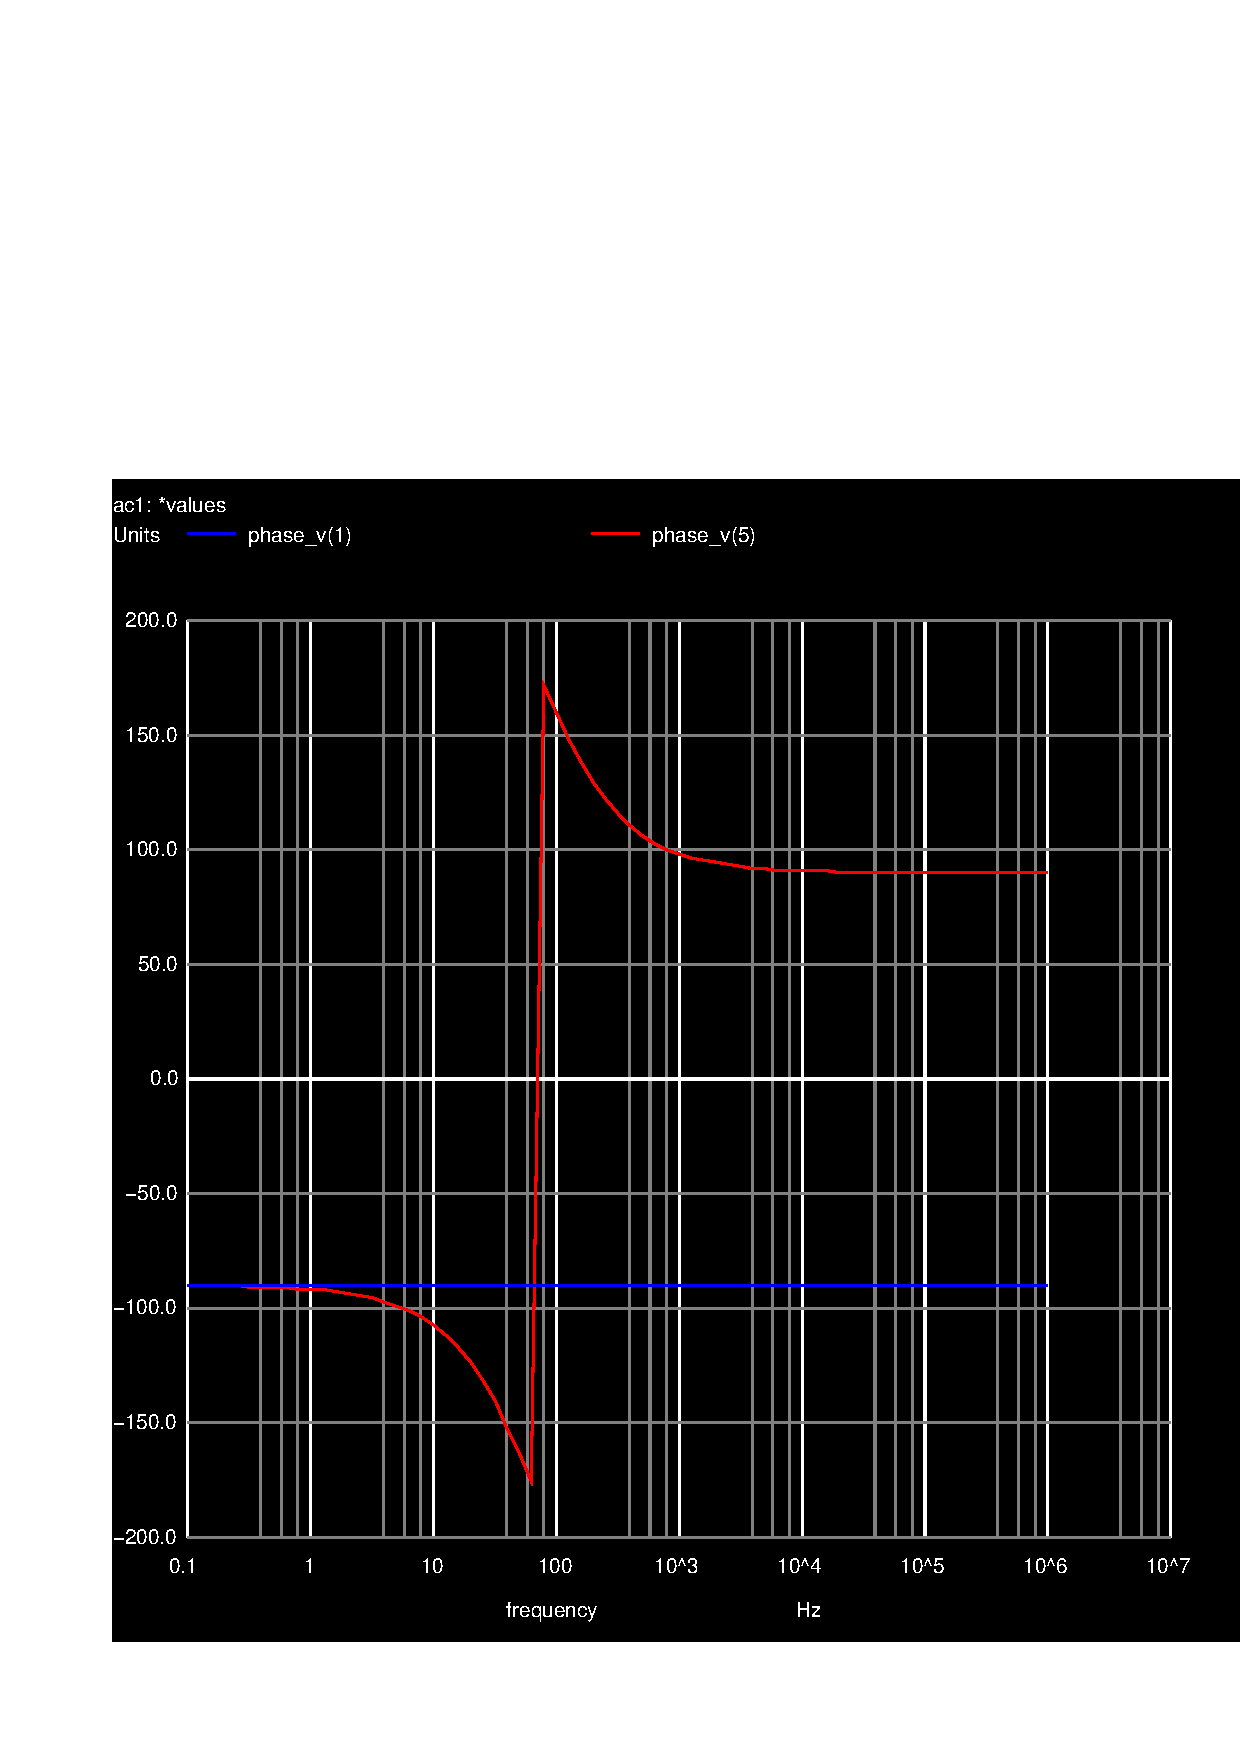
\includegraphics[scale=0.27]{phase.pdf}
\caption{Phase in order to frequency}
\label{fig:comparison 4}
\end{figure}
\FloatBarrier

\begin{table}[h]
\begin{center}
  \begin{tabular}{|c|c|}
    \hline    
    {\bf Name} & {\bf Value [Hz][Mu]} \\ \hline
    \input{../mat/data3_teo}
    \hline
  \end{tabular}
  \begin{tabular}{|c||c|}
    \hline    
    {\bf Name} & {\bf Value [Hz][Mu]} \\ \hline
    cost & 8.116008e+03\\ \hline
merit & 2.707518e+03\\ \hline

    \hline
  \end{tabular}
  \caption{Comparison 4}
  \label{tab:comparison 4}
\end{center}
\end{table}
\FloatBarrier


We can see that the cost is the same but the merit figure is higher using Ngspice's values, probably due to a higher bandwidth.

\section{Conclusion}
\label{sec:conclusion}

%All in all, this laboratory assignment showed that the difference between the theoretical models and the simulation is minimal, never differing more than one order of magnitude as seen in Section \ref{sec:sbs}. \par

%This lab assignment showed us that the main purpose of the bypass capacitor $C_E$ in the gain stage is to avoid a gain loss
%through resistor $R_E$ and the main purpose of resistor $R_E$ is to stabilize the temperature effect. In the DC component the temperature effect is most important while in AC the gain is. Therefore there needs to be an equilibrium, which is achieved by placing these components in parallel. \par
 
%Also, for lower frequencies (DC) capacitor $C_E$ behaves like an open circuit, so the current goes through resistor $R_E$, stabilizing the temperature effect. For higher frequencies (AC) the capacitor behaves like a short circuit and therefore it is used to bypass the resistor $R_E$ , avoiding a reduction of the gain (gain is stable in the desired passband). \par

%As for $R_C$, it increases the gain, so by playing with its value it is possible to achieve a better merit figure.



